\documentclass[12pt]{article}

\usepackage{graphicx}   % need for figures

% don't need the following. simply use defaults
\setlength{\baselineskip}{16.0pt}    % 16 pt usual spacing between lines

\setlength{\parskip}{3pt plus 2pt}
\setlength{\parindent}{20pt}
\setlength{\oddsidemargin}{0.5cm}
\setlength{\evensidemargin}{0.5cm}
\setlength{\marginparsep}{0.75cm}
\setlength{\marginparwidth}{2.5cm}
\setlength{\marginparpush}{1.0cm}
\setlength{\textwidth}{150mm}

\graphicspath{{../figures/}}

% above is the preamble

\begin{document}

\title{Assignment 3}
\author{William Richard}
\maketitle

\section{Regularized Linear Regression}

\subsection{How does $\lambda$ affect the results?}
As we would expect, for the train data, the MSE approaches the expected value as we increase $\lambda$.  On the test data, the MSE begins to approach the expected value, but at a very small $\lambda$ hits an inflection point and begins to go away from the expected MSE value.  This implies that, for larger $\lambda$, our model has overfit the data, and that the real model should have a small $\lambda$, i.e. a small regularization, and be trained mostly based on the actual trainin  data.

\subsection{How does the choice of $\lambda$ depend on the setting of features or number of examples?}

To explore how the number of examples affects the choice of $\lambda$, please compare figures \ref{fig:1-1000-100} and \ref{fig:1-150(1000)-100}.  Figure \ref{fig:1-150(1000)-100} clearly does better with a smaller $\lambda$ than figure \ref{fig:1-1000-100}.  With fewer examples, the 150(1000)-100 case becomes dominated by $\lambda$, and thus behaves better when $\lambda$ is smaller, or  having a smaller effect on the output.  Alternately, the 1000-100 case has many more examples, and thus can absorb the effects of a larger $\lambda$.  The large $\lambda$ has the added bonus of normalizing the data to a greater extent.

Next, compare figures \ref{fig:1-100-100} and \ref{fig:1-100-10} for the 100-100 and 100-10 cases, respectively.  These two figures would imply that with fewer features, in the 100-10 case, a lower $\lambda$ is better.

\begin{figure}[h]
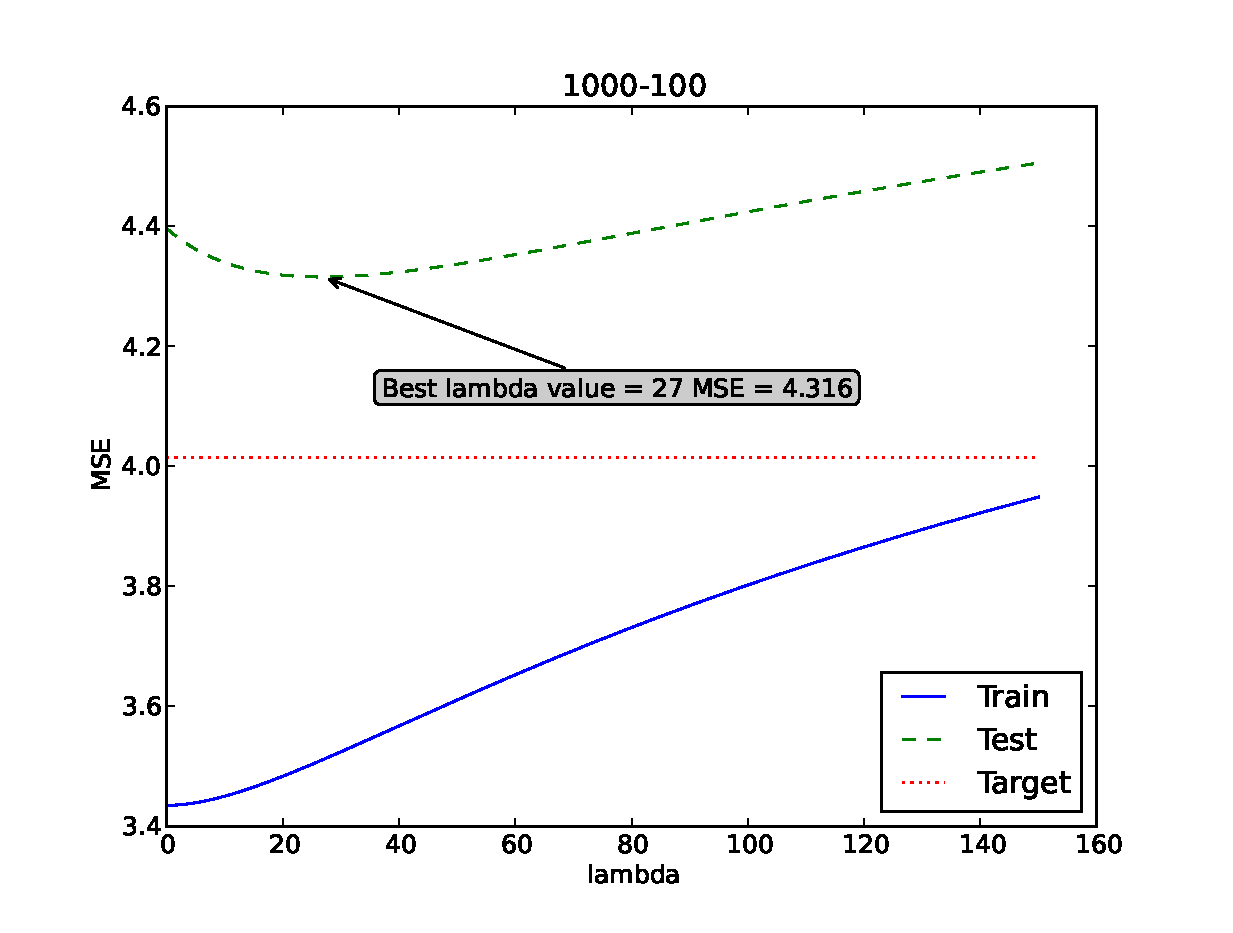
\includegraphics[height=.5\textheight]{1/1000-100.eps}
\label{fig:1-1000-100}
\caption{Regularized Linear Regression on 1000-100}
\end{figure}

\begin{figure}[h]
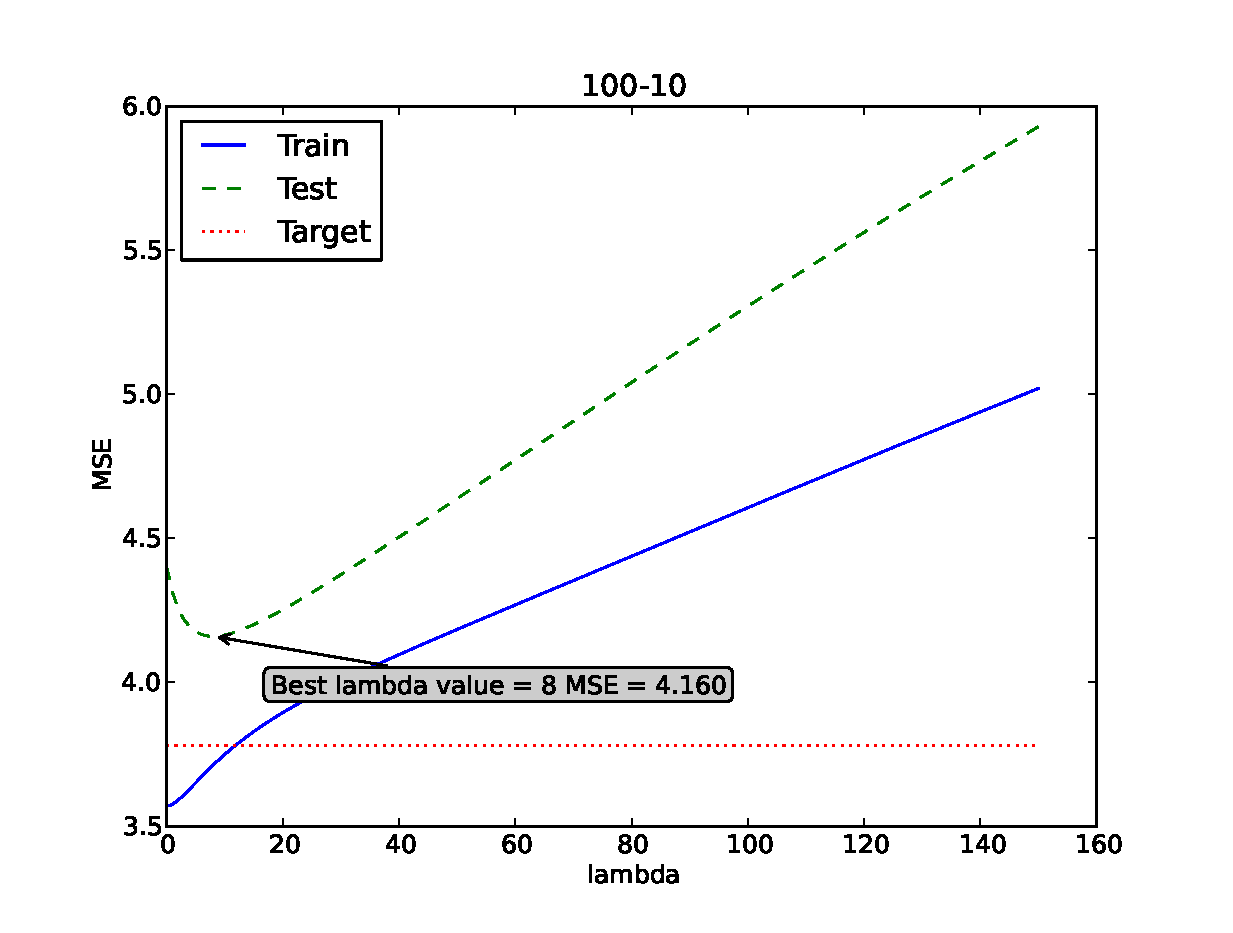
\includegraphics[height=.5\textheight]{1/100-10.eps}
\label{fig:1-100-10}
\caption{Regularized Linear Regression on 100-10}
\end{figure}

\begin{figure}[h]
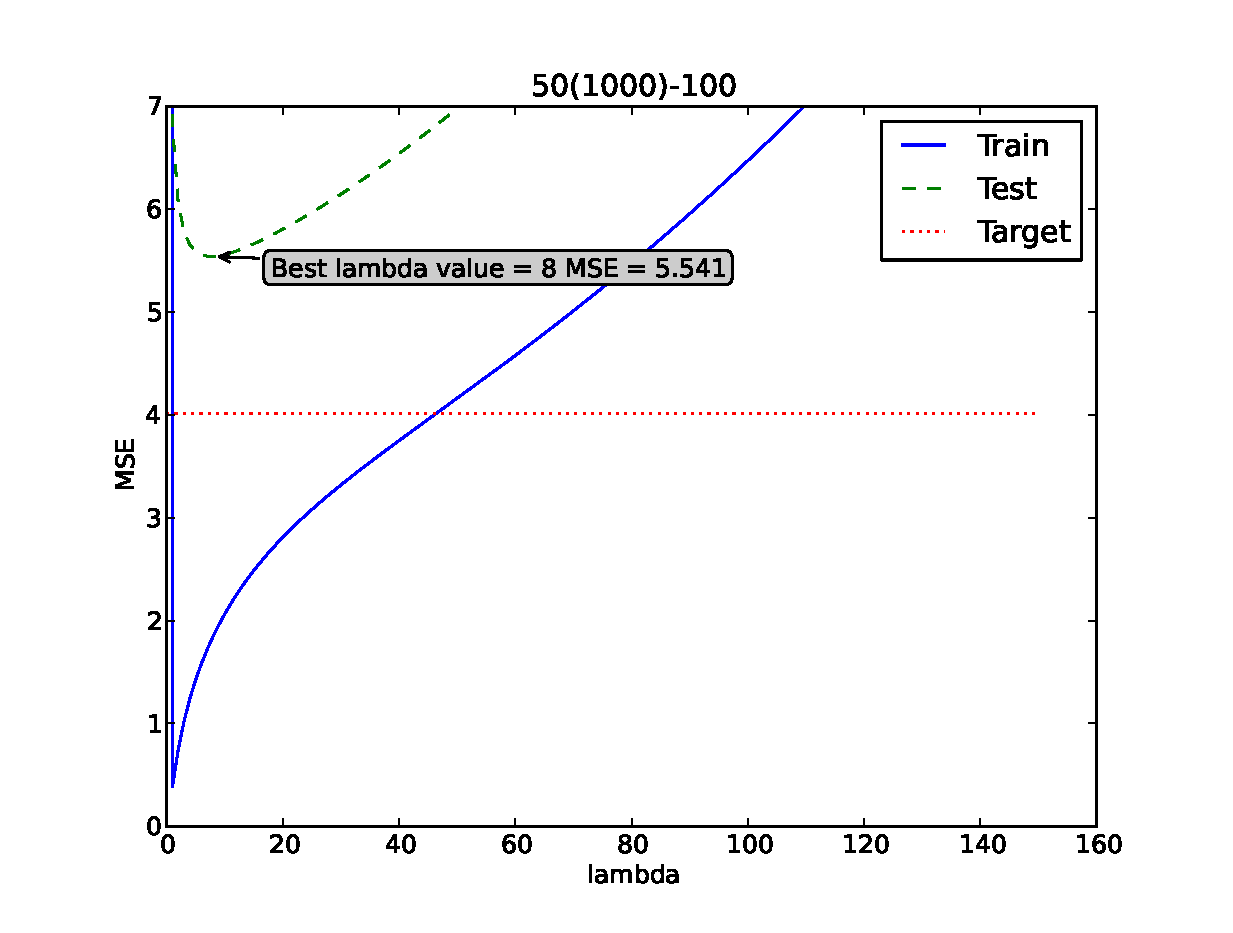
\includegraphics[height=.5\textheight]{1/50(1000)-100.eps}
\label{fig:1-50(1000)-100}
\caption{Regularized Linear Regression on 50(1000)-100}
\end{figure}

\begin{figure}[h]
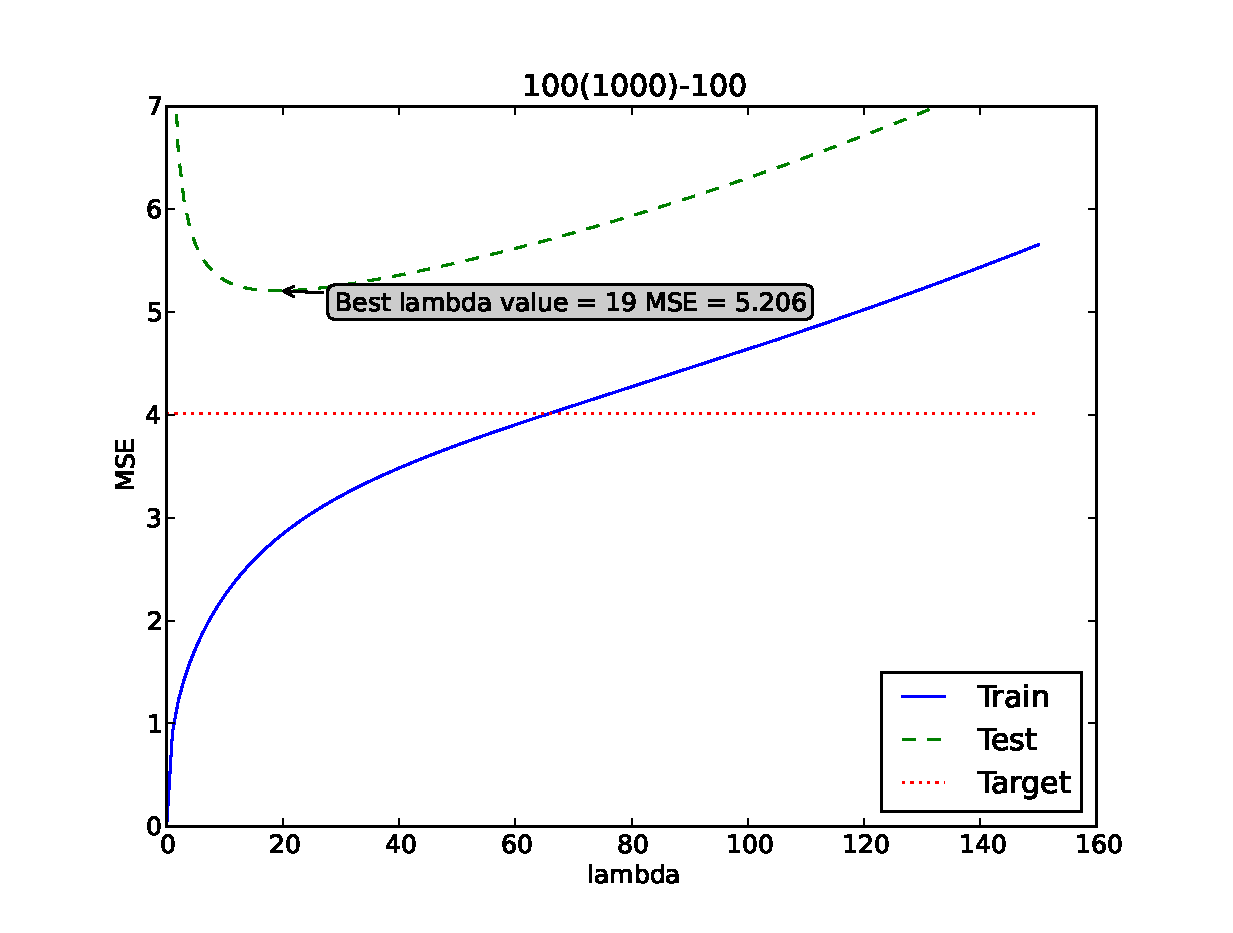
\includegraphics[height=.5\textheight]{1/100(1000)-100.eps}
\label{fig:1-100(1000)-100}
\caption{Regularized Linear Regression on 100(1000)-100}
\end{figure}

\begin{figure}[h]
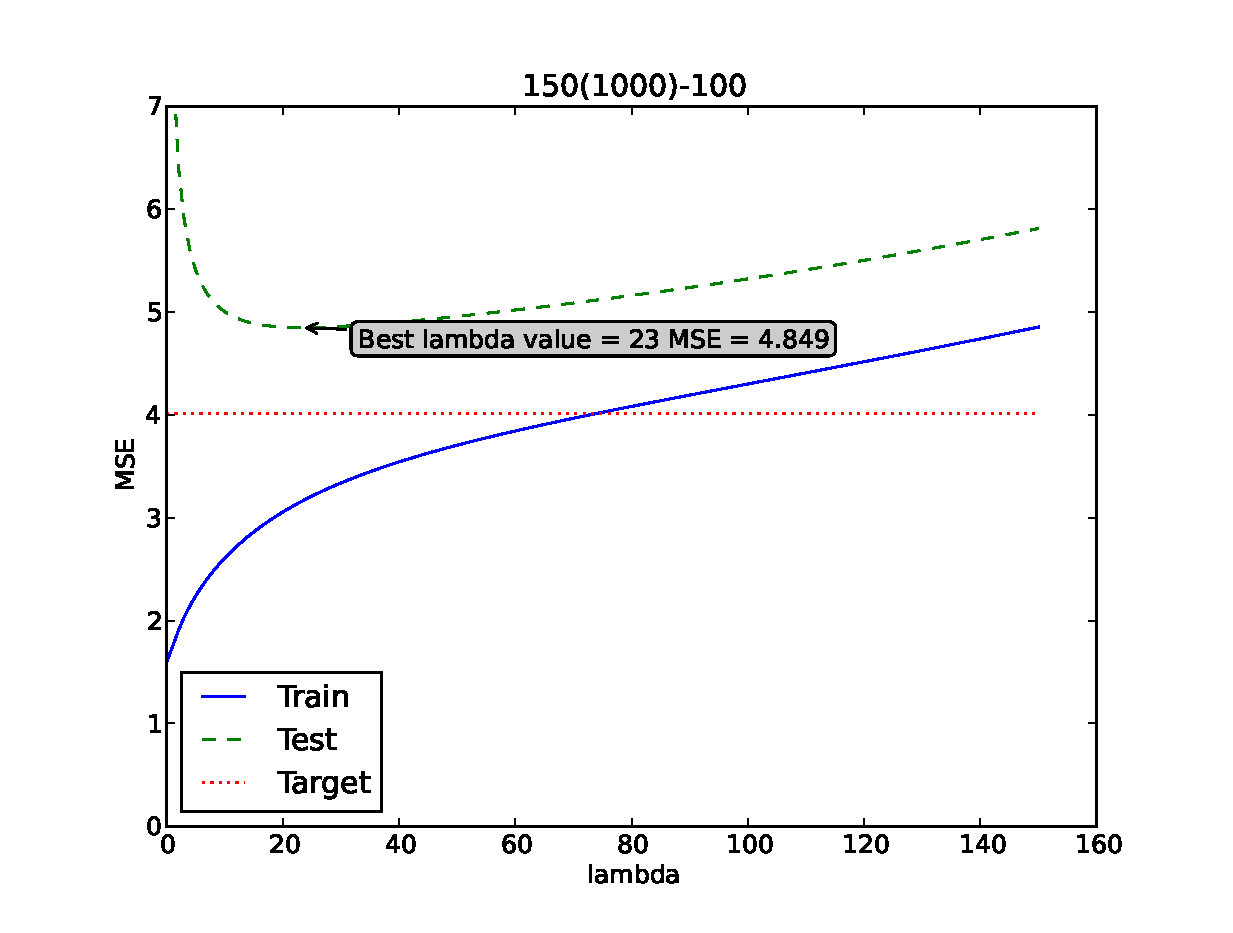
\includegraphics[height=.5\textheight]{1/150(1000)-100.eps}
\label{fig:1-150(1000)-100}
\caption{Regularized Linear Regression on 150(1000)-100}
\end{figure}

\begin{figure}[h]
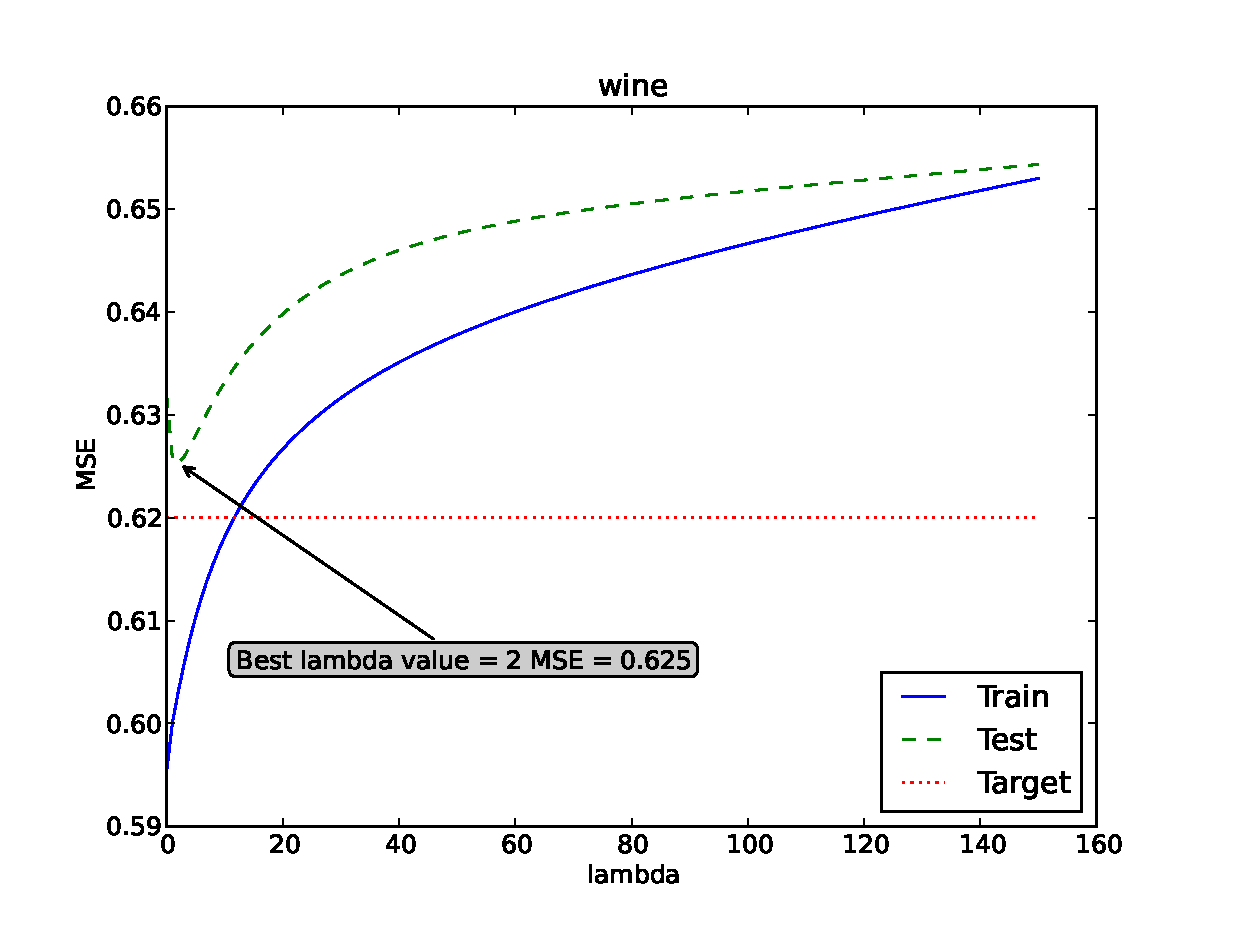
\includegraphics[height=.5\textheight]{1/wine.eps}
\caption{Regularized Linear Regression on wine}
\label{fig:1-wine}
\end{figure}

\begin{figure}[h]
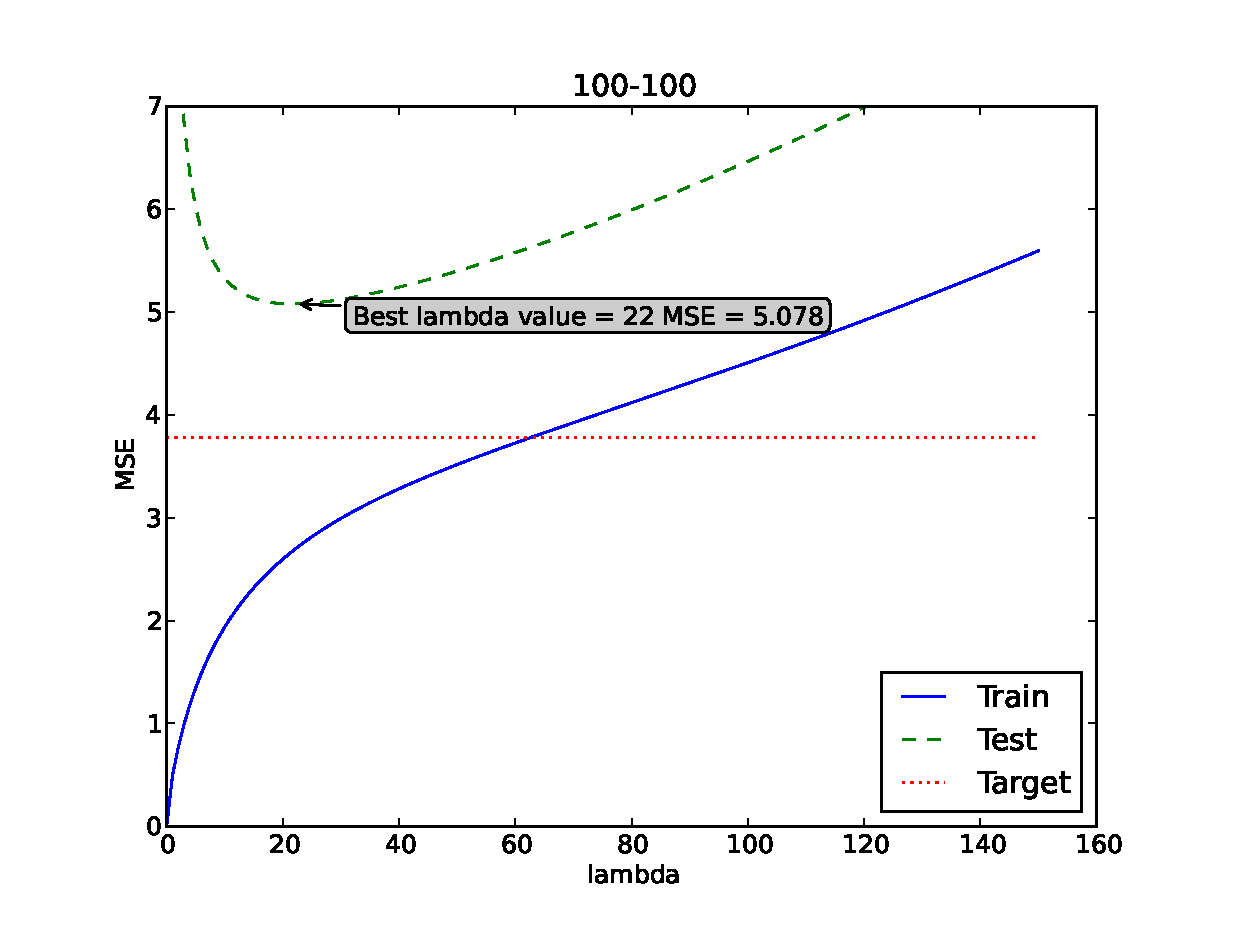
\includegraphics[height=.5\textheight]{1/100-100.eps}
\caption{Regularized Linear Regression on 100-100}
\label{fig:1-100-100}
\end{figure}

\section{Learning Curves}
\begin{figure}[h]
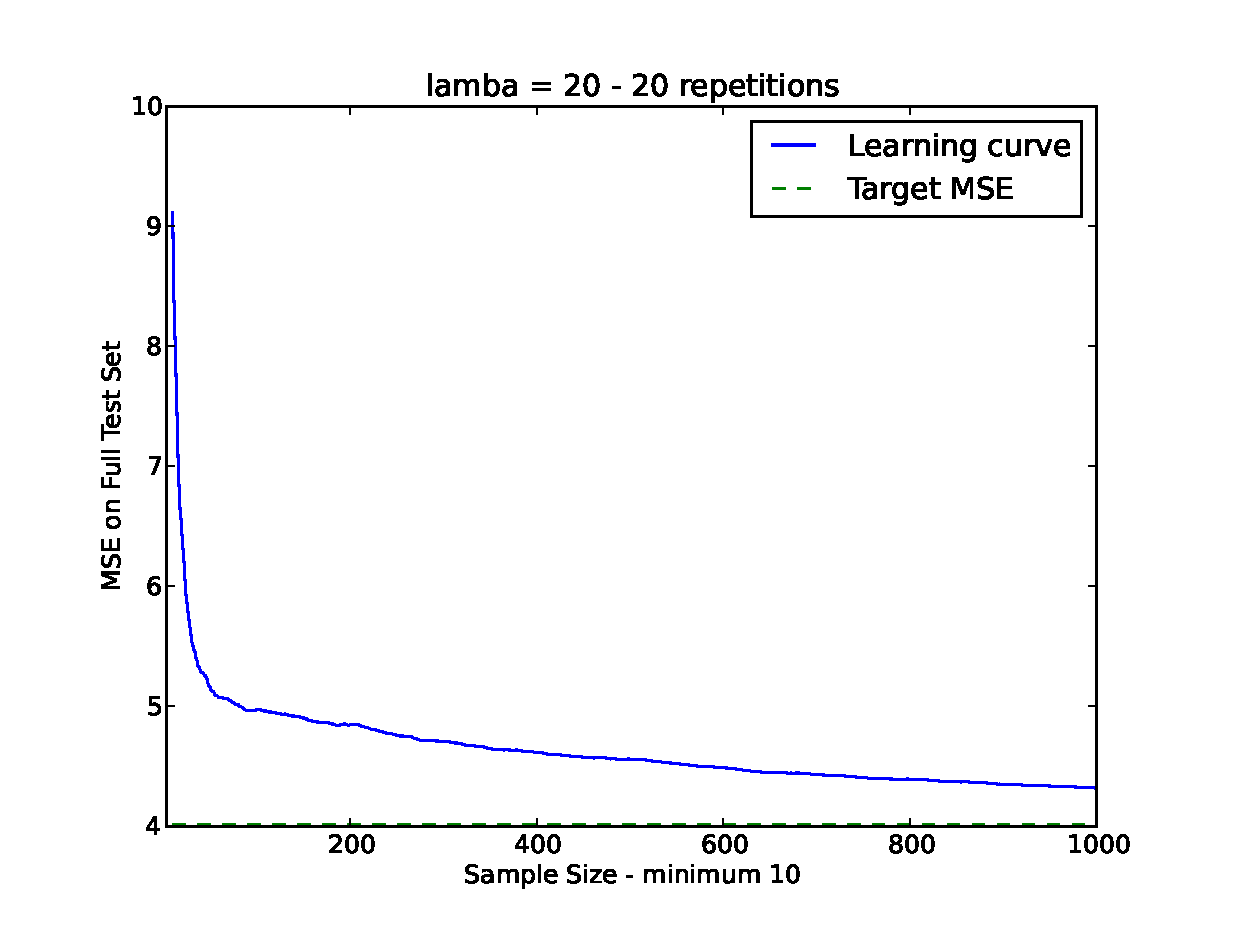
\includegraphics[height=.5\textheight]{2/1000-100-20-20-problem2.eps}
\label{fig:2-20}
\caption{Learning Curve for 1000-100 with Lambda = 20}
\end{figure}
\begin{figure}[h]
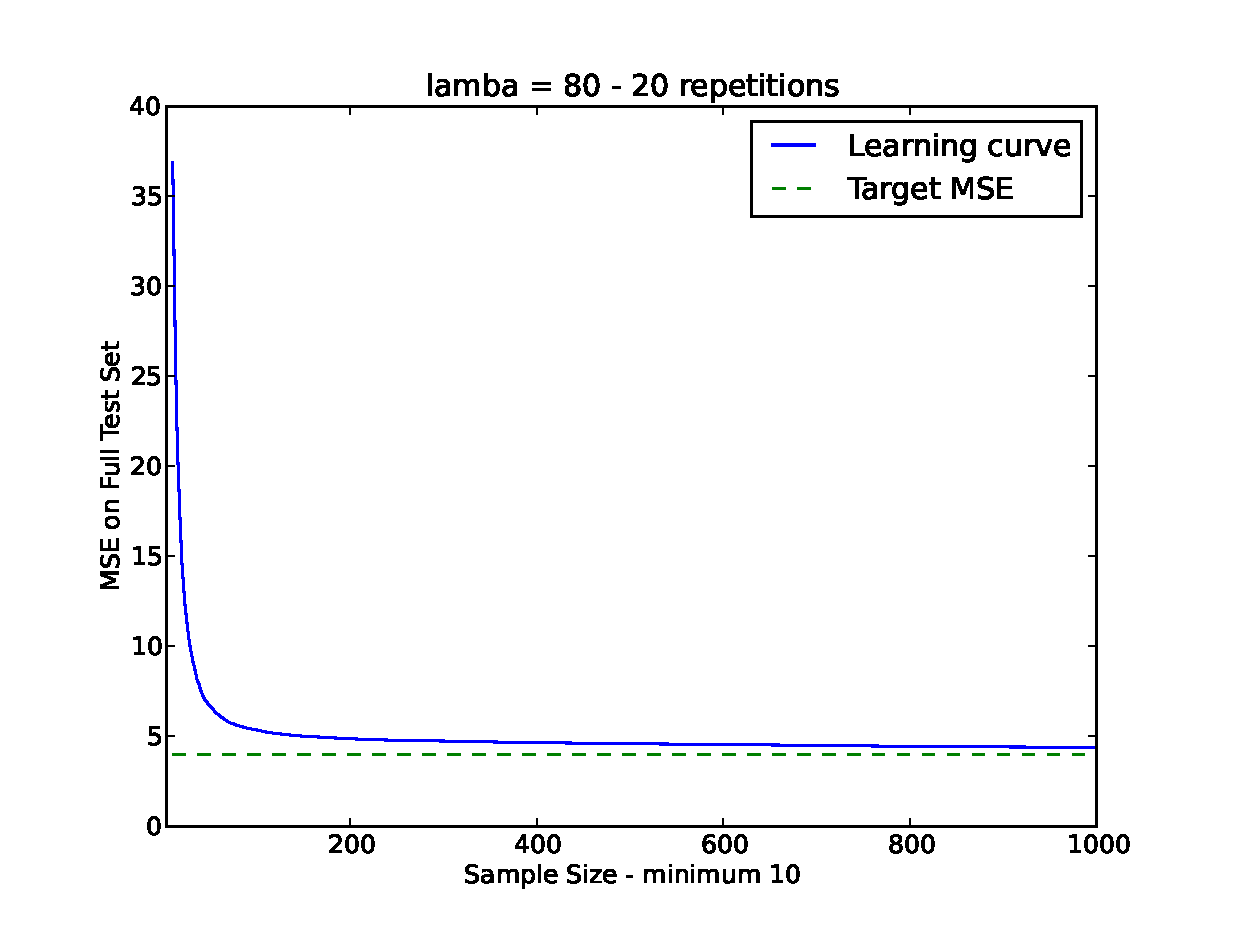
\includegraphics[height=.5\textheight]{2/1000-100-80-20-problem2.eps}
\label{fig:2-80}
\caption{Learning Curve for 1000-100 with Lambda = 80}
\end{figure}
\begin{figure}[h]
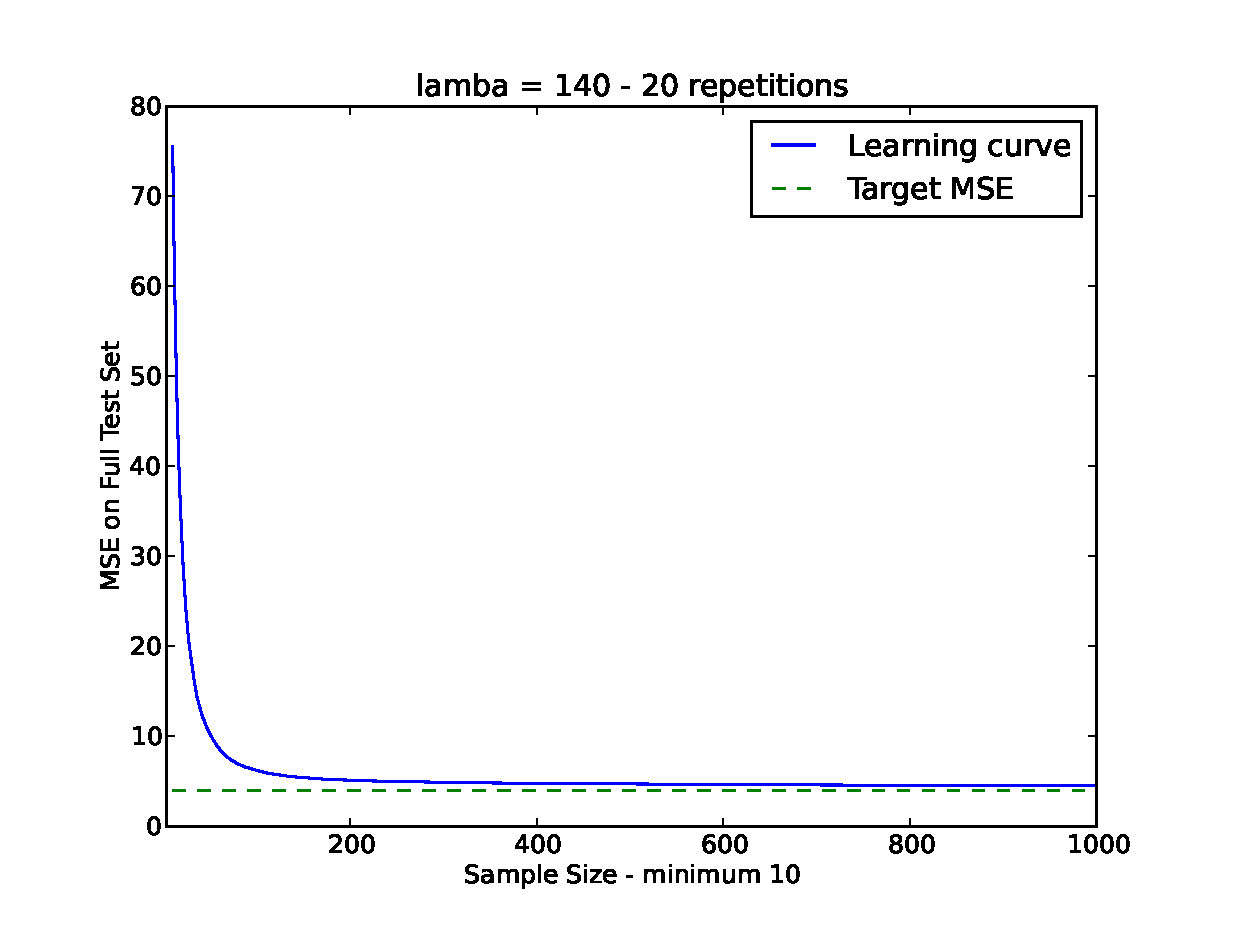
\includegraphics[height=.5\textheight]{2/1000-100-140-20-problem2.eps}
\label{fig:2-140}
\caption{Learning Curve for 1000-100 with Lambda = 140}
\end{figure}

With the larger $\lambda$ values, you see much faster stabilization of MSE value with respect to sample size.  This occurs because, with larger $\lambda$, indivdual samples are normalized more, thus there is less noise, and the data matters less, resulting in faster convergence to the final MSE value.

\section{Cross Validation}

\begin{table}[h]
\begin{tabular}{c||p{3cm}|p{3cm}||p{3cm}|p{3cm}}
Data Set & Cross Validation  &  & Reg. Lin. Regression &  \\
 & $\lambda$ & MSE & $\lambda$ & MSE \\
\hline
50(1000)-100 & 24 & 5.3 & 8 & 5.541\\
100(1000)-100 & 30 & 4.840 & 19 & 5.206 \\
150(1000)-100 & 46 & 4.869 & 23 & 4.849 \\
1000-100 & 39 & 4.137 & 27 & 4.316 \\
100-10 & 12 & 4.159 & 8 & 4.160\\
100-100 & 20 & 4.494 & 22 & 5.078\\
wine & 3 & 0.642 & 2 & .0625\\
\end{tabular}
\label{tab:3}
\end{table}

In most of the data sets, especially the ones with a large number of examples, the $\lambda$ that was chosen using regularized linear regression was close to the $\lambda$ chosen using cross validation.  When cross validation gave a different result than regularized linear regression, cross validation has produced a vastly superiour result.

Based on the 50(1000)-100, 100(1000)-100, 150(1000)-100 and 1000-100 series, it seems that cross validation does better with more examples, but this falls directly from regularized linear regression doing better with more examples.  Since you're using the same algorithm, if regularized linear regression does better with more examples, cross validation will do better with more examples.

Comparing the 100-10 and 100-100, it seems to be the case that when you have fewter features, cross validation doesn't give as much of an improved result.  That said, this is based on only one data point, and it could easly be luck that cross validation did not have a better result for the 100-10 data set.  The evidence is not conclusive that number of features has an effect on the results of cross validation.

Refer to table \ref{tab:runtimes} for the runtimes of the various problems for all of the data sets.  It is immediately aparent that cross validation takes much more time that conventional linear regression.  This is obvious from the algorithm - you're essentially doing the same calculation, but ten times instead of once.  The results are superior, but at a steep computational cost.


\begin{table}
\label{tab:runtimes}
\caption{Average runtime of 5 runs, in seconds}
\begin{tabular}{c|c|c|c}
Data Set & Regularized L.R. & Cross Validatien & Bayesian L.R \\
\hline
1000-100 & 5.813 & 31.730 & 0.135 \\
50(1000)-100 & 2.297 & 4.720 & 0.071 \\
100(1000)-100 & 2.325 & 6.247 & 0.0486 \\
150(1000)-100 & 2.707 & 7.889 & 0.0540 \\
100-10 & 2.229 & 1.937 & 0.0174 \\
100-100 & 2.492 & 6.145 & 0.0.417 \\
wine & 6.948 & 5.0199 & 0.0673 \\
\end{tabular}
\end{table}

\section{Bayesian Linear Regression}
\begin{table}[h]
\begin{tabular}{c|c|c|c||c|c}
Data Set & $\alpha$ & $\beta$ & MSE & Cross Validation MSE & Target MSE\\
\hline
100-10 & 1.201 & 0.256 & 4.180 & 4.159 & 3.78\\
100-100 & 1.082 & 0.509 & 7.547 & 4.494 & 3.78\\
50(1000)-100 & 0.978 & 0.345 & 5.811 & 5.3 & 4.015\\
100(1000)-100 & 1.361 & 0.307 & 5.739 & 4.840 & 4.015\\
150(1000)-100 & 1.665 & 0.266 & 5.243 & 4.869 & 4.015\\
1000-100 & 2.733 & 0.264 & 4.338 & 4.137 & 4.015 \\
wine & 6.084 & 1.610 & 0.627 & 0.642 & \\
\end{tabular}
\label{tab:4}
\end{table}

If we examine the 1000-100 data set and its subsets, it is clear that Bayesian Linear Regression does better with more examples.  The trend is clear and distinct.

It appears that Bayesian Linear Regression does better with fewer features, based on how much better the 100-10 data set's results were than the results from the 100-100 data set.

\section{Comparison of Algorithms}

As we've discussed earlier, Cross Validation is superior to Regularized Linear Regression for two reasons.  Firstly, Cross Validation outperforms Regularized Linear Regression.  Secondly, you only discover the optimal result of Regularized Linear Regression after you look at the answers from the test set.

Cross validation outperformed Bayesian Linear Regression in every case, as you can see in table \ref{tab:4}.  But, as we can see in tabe \ref{tab:runtimes}, Bayesian Linear Regression is orders of magnitude faster.  Furthermore, if there are many examples, the results of Bayesian Linear Regression are comparable to Cross Validation.  This implies that there are some cases where Bayesian Linear Regression may be the superior algorithm.  If you require an algorithm that trains quickly on new data, and your data sources have many examples, then Bayesian Linear Regression is definately the correct choice.  But, if you have unlimited time to train your model, or your data set is small, it appears like Cross Validation would be the better algorithm.

\end{document}